\documentclass[12pt]{article}
\usepackage[margin=1in]{geometry}
\usepackage{listings}
\usepackage{amsmath}
\usepackage{amsfonts}
\usepackage{fancyvrb}
\usepackage{minted}
\usepackage{graphicx}
\usepackage{tikz}
\usepackage{enumitem}  %this permits the enumeration items to flow past sections
% Set vertical space between paragraphs
\setlength{\parskip}{1cm}

% Set paragraph indentation
\setlength{\parindent}{1cm}

\title{Algorithms - Assignment 6}
\date{Due Thursday, March 28th by 11:59 pm}

\begin{document}
\maketitle

\begin{enumerate}
    \item[(1)] Perform Dijkstra's shortest paths algorithm on the following graph (graph $\alpha$) with $A$ as the starting node. Along the way you should
    \begin{itemize}
        \item[(a)] Create a table showing the intermediate distance values of all nodes after each iteration of the algorithm (i.e. there should be a column for each time a new node is released from the priority queue, and a row for every node). Make sure to include an extra column and row labelling everything (i.e. have an `A' left of the A row, a 1 above the first iteration column, etcetera), so the graders can understand what they are looking at. Alongside these distances you should also include the current best predecessor (i.e. the \emph{prev} values associated with each node). You don't need to include the state of the priority queue after each iteration, but you will almost certainly need to write it down on paper in order to carry out the algorithm.
        \item[(b)] Afterwards, draw the shortest-paths tree. 
    \end{itemize}
    \begin{figure}[h]
        \centering
        \includegraphics[width=1\textwidth]{hw6_graph1.png}
        \caption{Graph $\gamma$}
    \end{figure}

    \item[(2)] Consider a pixel map of a tropical archipeligo (figure $\alpha$), like figure $\alpha$ which I absolutely did not steal from somewhere else.
        \begin{figure}[h]
            \centering
            \includegraphics[width=0.4\textwidth]{island_problem.png}
            \caption{Figure $\alpha$}
        \end{figure}
    The gray tiles represent land, while the blue tiles represent ocean. We want an algorithm which, given this map in the form of an $n \times n$ matrix of $0$s and $1$s ($0$ representing water, $1$ representing land), returns the number of distinct islands. We will consider two tiles to be a connected landmass if they are adjacent to one another (this will include corners touching, so all 8 tiles surrounding a tile should be considered adjacent). Describe using words and pseudocode (but don't actually program unless you want to) an algorithm which does this. \par 
    
    Your algorithm should work in linear time with respect to the number of cells (so if we have a square $n \times n$ matrix as input, linear runtime would actually be $O(n^2)$, not $O(n)$). Be clear about how you are representing this as a graph problem, and how your graph would be represented in code. \par 
    
    (\emph{Hint:} This problem really should have been on the previous homework, although both breadth-first and depth-first searches can work here. Try and express this as a graph connectivity problem.)
    \item[(3)] Consider the 8x8 chess board pictured below. The red circle represents a knight chess piece, and the 8 X marks represent the different legal moves that a knight can make. To represent position on the board: top-left cell will be position $(0,0)$, bottom left will be $(0,7)$, top right will be $(7,0)$, and bottom right will be $(7,7)$. Our problem will deal with a \emph{generalized} chess board, i.e. an $n \times n$ grid, but with the same convention for representing positions. \par 
    \begin{itemize}
        \item[(a)] Write a python function which, given the dimension of the game board $n$, an initial position, and a destination position, returns the minimum number of moves that a knight needs to make in order to move from that initial position to the final position, \emph{as well as} a specific sequence of moves which will get them to that position. (Represent the moves with two-letter strings, i.e. `ul' should represents moving two cells up and one cell left.) \par 
    
        You'll want to use breadth first search for this, but I like this exercise because the actual graph will be \emph{implicit} to your solution: don't try to force an adjacency list into your code. I recommend making a helper function which calculates the resulting position of a move applied to a knight in a given position (or an error code if the move is invalid), and then using that function in order to check for `edges'. As a quick way of checking your program, the minimum number of moves required to travel from the position (0,7) to (7,0) is six, and there are many possible ways of getting there in this many moves (some of which might surprise you). Don't jump to thinking your program is wrong if the path it returns looks weird at first (like I did).
        \item[(b)] What is the runtime with respect to $n$?
    \end{itemize}
    \begin{center}
        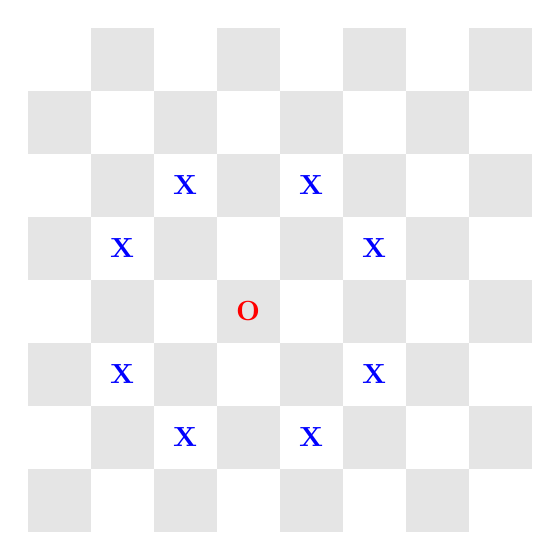
\begin{tikzpicture}[scale=0.8]
            % Draw chessboard
            \foreach \i in {0,...,7} {
                \foreach \j in {0,...,7} {
                    \pgfmathtruncatemacro{\shade}{mod(\i+\j,2)}
                    \ifnum\shade=0
                        \fill[black!10] (\i,\j) rectangle ++(1,1);
                    \fi
                }
            }
            
            % Draw knight's moves from position d4
            \foreach \i/\j in {1/2, 2/1, 2/3, 1/4, 3/2, 3/4, 4/1, 4/3} {
                \pgfmathtruncatemacro{\x}{3 + \i}
                \pgfmathtruncatemacro{\y}{3 + \j}
            }
            
            % Draw starting position
            \node at (3.5,3.5) {\textcolor{red}{$\mathbf{O}$}};
            \node at (4.5,5.5){\textcolor{blue}{$\mathbf{X}$}};
            \node at (2.5,5.5){\textcolor{blue}{$\mathbf{X}$}};
            \node at (1.5,4.5){\textcolor{blue}{$\mathbf{X}$}};
            \node at (1.5,2.5){\textcolor{blue}{$\mathbf{X}$}};
            \node at (2.5,1.5){\textcolor{blue}{$\mathbf{X}$}};
            \node at (4.5,1.5){\textcolor{blue}{$\mathbf{X}$}};
            \node at (5.5,2.5){\textcolor{blue}{$\mathbf{X}$}};
            \node at (5.5,4.5){\textcolor{blue}{$\mathbf{X}$}};
        \end{tikzpicture}
    \end{center}
    \item[(2)] In this problem, you will use the priority queue data structure that you created in homework 4 in order to implement Dijkstra's algorithm. 
    \begin{itemize}
        \item[(a)] Before that though, we need to make a few changes/additions to it (I tried to leave you with something which would be perfect for Dijkstra in that homework, but my planning was not perfect.) Don't worry, this part shouldn't take long.
        \begin{itemize}
            \item Replace the increase\_priority(self, task, k) function with a function called change\_priority(self, task, k). Instead of adding k to the current priority, it should simply replace the old priority with k. This is better suited for Dijkstra. 
            \item The biggest addition we need to make is that our priority queue needs a min-mode, in which the lowest numbers have the highest priority. We can do this in same way that we talked about turning a max-heap into a min-heap. 
            
            In the constructor, add an additional default argument called mode, which defaults to the string `max'. The constructor should initialize an attribute of the same name to that argument. (I.e. add the line self.mode = mode). 

            All we need to change in order to make everything work in min-mode is add a few checks to the enqueue(self, task, priority), dequeue(self, task, priority), and change\_priority(self, task, k) methods. For enqueue, simply add a check which multiplies the input priority by -1 if the mode attribute is set to `min' before using it. This will make it so that behind the scenes, all of the priorities will be negative, although the user will never actually see this. When the user dequeues something, they should have their original priority returned, not the negative priority, so add a mode check to that method which multiplies by -1 again before returning the when in min-mode. Finally, in the change\_priority method, add a mode check which multiplies k by -1 when in min-mode before using it. That should be all you need to change in order to switch your priority queue between a max mode and a min mode. 
            \item We will add two more dunder methods which aren't strictly necessary, but will your queue easier to work with and thus make Dijkstra a little more straightforward to implement. These are \_\_len\_\_(self) and \_\_contains\_\_(self, task). The first is what python looks for when len(thing) is called. Have your queue return the size of the underlying heap when len(Q) is called (one line of code). \_\_contains\_\_(self, task) is what python looks for when you write an if statement that checks for membership. I.e.
            \begin{minted}{python3}
                l = [1,2,3,4]
                if 1 in l: print("Found it")
            \end{minted}
            When python sees the `in' here, it looks for a method called \_\_contains\_\_(1), which is supposed to return a True or False value. Make such a method check to see if a task is currently in the queue (you can do this in constant time using the data\_locations dictionary attribute). 
        \end{itemize}
        \item[(b)] With that out of the way, your queue should be ready for use in Dijkstra. Program it the way we discussed in class. Your function dijkstra(G,s) should take two arguments, a weighted graph G and a starting node s. Further instructions:
        \begin{itemize}
            \item The graph should be a weighted adjacency list in the form of a dictionary of dictionaries. Rather than try to explain what exactly that means here, I've included an example graph on canvas. This graph I've included is precisely the graph from question 1 of this assignment. You already know what the output should be for this graph, so you can use it to see if your code is working.
            \item Have the starting node $s$ default to the first node in the adjacency list. After that and before doing anything else, your function should test to see if the starting node is an actual node in the graph. If it isn't, then return an error message and stop.
            \item The function should return two outputs: dists, a dictionary of shortest distances to $s$ for each node, and prevs, a dictionary of predecessors in the shortest paths tree, so that shortest paths can be recovered. 
        \end{itemize} 
    \end{itemize}
    \item[(4)] 
    \begin{itemize}
        \item[(a)] Now implement Bellman-Ford in python. It should take identical inputs as your function for Dijkstra did (a weighted adjacency list and a starting node) and return the same predecessor and distance dictionaries. Remember: Bellman-Ford is a brute(ish) force algorithm, and shouldn't be difficult to program. Mine only amounted to about 20 lines of code (same for Dijkstra, excluding the priority queue). You can assume that all edge weights are positive, and so there is no need for programming negative cycle detection. 
        \item[(b)] I've included on canvas a python function which generates random graphs (with positive edge weights). Use this to run some tests comparing Bellman-Ford with Dijkstra, creating plots in MatPlotLib like usual. You should see Dijkstra massively outperforming Bellman-Ford. Remember though that Bellman-Ford still has its uses: it works when there are negative edge weights, unlike Dijkstra. 
    \end{itemize}
    
\end{enumerate}


\end{document}